




\section{\ours Pipeline}
\label{sec:method}
As a monocular dense SLAM pipeline (\cref{fig:architecture}), our aim is to simultaneously track camera poses and reconstruct the recorded scene online using a dense pointcloud. To achieve this, we propose a lightweight and novel symmetric two-view association model as the frontend of our pipeline, which extracts the relative pose and local point maps of two neighboring input frames (\cref{subsec:frontend} and \cref{subsec:loss}). In the backend, a sparse and efficient $\mathrm{Sim}(3)$ pose graph optimization with loop closure is performed to mitigate drift accumulation (\cref{subsec:backend}).

\subsection{Symmetric Two-view Association Model}\label{subsec:frontend}
In classical monocular SLAM pipelines, the two-view estimation is one of the most critical building block, as it establishes geometric constraints that allow for further optimization. In this work, we follow the same principle; however, instead of relying on traditional methods, we propose a deep learning based Symmetric Two-view Association (STA) model that eliminates the need for camera intrinsics in the SLAM process. %As shown in \cref{fig:symmetric}, comparing to previous two-view models~\cite{dust3r,mast3r}, our symmetric design reduces the size from 0.7B to 0.4B.

\boldparagraph{Encoder}
Our STA model takes in two images $\bm{I}_i$, $\bm{I}_j$ as input. It uses a shared ViT encoder~\cite{dosovitskiy2020image} to divide input images into patches and encode them into features
\begin{equation*}
    \bm E_{i/j} = \text{Encoder}\left(\bm I_{i/j}\right) \quad \in \mathbb{R}^{K\times C},
\end{equation*}
where $K$ represents tokens and $C$ denotes the dimensions. Subsequently, we insert a camera pose embedding $\bm p$ to the encoding features of each view, forming
\begin{equation*}
    \bm E'_{i/j} = \left(\bm p, \bm E_{i/j}\right) \quad \in \mathbb{R}^{(K+1)\times C}.
\end{equation*}


\boldparagraph{Decoder}
The decoder further processes and fuses information between the encoding features $\bm E'_i$ and $\bm E'_j$. It contains a sequence of $B$ decoder blocks, each conducting a self-attention operation followed by a cross-attention operation, producing decoding features
\begin{align*}
\bm D_{i/j}^{(b)} &= \text{DecoderBlock}^{(b)} \left(\bm D_{i/j}^{(b-1)}, \bm D_{j/i}^{(b-1)}\right) \in \mathbb{R}^{(K+1) \times C'},
\end{align*}
where $b \in \left\{1, 2, \dots, B\right\}$ is the index of a decoder block, and $\bm D_{i/j}^{(0)}=\bm E'_{i/j}$.


\boldparagraph{Symmetric Formulation}
Prior approaches~\cite{dust3r,mast3r} regress both point maps into the coordinate frame of the first view, thus requiring two separate decoders. In contrast, our model predicts only local point maps and relative poses between views. This fully symmetric formulation makes it possible to use only one decoder. As a result, the number of parameters for decoding is effectively reduced by half (shown in \cref{fig:symmetric}), forming a more compact model for real-time applications. Moreover, producing local view outputs in their own coordinate systems is better suited for the subsequent pose graph optimization, see \cref{subsec:backend} for details.

\boldparagraph{Local Point Maps}
Given decoding features $\bm D_{i/j}^{(b)}$, we use a DPT head~\cite{ranftl2021vision} to regress the local point maps $\bm P$ and corresponding confidence maps $\bm W$:
\begin{align*}
    \bm P_{i/j}, \bm W_{i/j} = \text{PointHead}\left(\bm D_{i/j}^{(b)}\right)
\end{align*}


\boldparagraph{Relative Poses}
% The first token $\bm p_i$ and $\bm p_j$ of the decoder output $\bm D_i^{(B)}$ and $\bm D_j^{(B)}$ will be used to regress the relative pose, while the rest of the tokens $\bm F^i$ and $\bm F^j$ will be used for local point maps.
% We will show later that our predictions are defined either in the local coordinate system of each view or relative to the other view.
Given the first embedding of the decoding feature $\bm D_i^{(B)}$, i.e., the camera pose embedding $\bm{p}_i^{(B)} \in \mathbb{R}^{1\times C'}$, we use an MLP to regress the relative transformation from view $i$ to $j$ . Specifically, the MLP outputs a matrix $\bm M_{ij} \in \mathbb{R}^{3\times 3}$ for rotation, a translation vector $\bm t_{ij} \in \mathbb{R}^{3\times1}$, and a confidence score $w_{ij} \in [0,1]$:
\begin{equation*}
    \bm M_{ij}, \bm t_{ij}, w_{ij} = \text{PoseHead}(\bm p_i^{(B)})
\end{equation*}
Since $\bm M_{ij}$ is not guaranteed to lie on the $SO(3)$ manifold, we apply SVD orthogonalization~\cite{levinson2020analysis} to it to obtain a valid rotation matrix $\bm R_{ij}$.
Then, the relative transformation is $\bm T_{ij} = \left[\bm R_{ij} | \bm t_{ij}\right]$.
With our symmetric formulation, we could also input $\bm p_j$ into the pose head to regress $\bm T_{ji}$. But in practice we only regress one of them for building pose graph.

\subsection{Training Objective}
\label{subsec:loss}
There are three loss terms to supervise the training of our STA model. \textit{Pointmap Loss} compares the regressed local pointmap with ground-truth points. \textit{Relative Pose Loss} penalizes errors in relative rotation and translation, with a cycle-consistency term ensuring the two predicted poses are mutual inverses. \textit{Geometric Consistency Loss} enforces alignment of the two local point maps after applying the predicted relative transformation, improving local reconstruction consistency.


\boldparagraph{Local Pointmap Loss}
Following DUSt3R~\cite{dust3r}, we apply the confidence-weighted regression loss for all predicted point maps with valid ground truths. Since the reconstruction is up-to-scale, we also normalize the regressed pointmap and the ground-truth pointmap according to their mean Euclidean distance to the origin, $n$ and $\hat{n}$:
% \begin{align}
% L_\text{pmap} = \sum_{x=\{i,j\}} & \|\bm W_x^{\text{point}}\odot(\hat{\bm P}_x^{\text{norm}} - \bm P_x^{\text{norm}})\|   \nonumber\\
% &- \alpha^{\text{point}}\log(\bm W^{\text{point}}_x),
% \end{align}
% \begin{align}
% L_\text{pmap} = \sum_{\substack{0 \leq u < W \\ 0 \leq v < H}} & \left\|\bm W_{i/j}(u,v)\odot \left(\frac{\hat{\bm{P}}_{i/j}(u,v)}{\hat{n}} - \frac{\bm{P}_{i/j}(u,v)}{n} \right)\right\|   \nonumber\\
% &- \alpha^{\text{point}}\log\left(\bm W_{i/j}(u,v)\right),
% \end{align}
\begin{align}
L_\text{pmap} = \sum_{v \in \{i, j\}} \sum_{\bm x \in \bm{I}_v} & \left\|\bm W_v(\bm x)\cdot \left(\frac{\hat{\bm{P}}_v(\bm x)}{\hat{n}} - \frac{\bm{P}_v(\bm x)}{n} \right)\right\|   \nonumber\\
&- \alpha^{\text{point}}\log\left(\bm W_v(\bm x)\right),
\label{eq:loss_pmap}
\end{align}
where $x$ is the pixel coordinate. Note that all the points are regressed in the local coordinate space of each view.

\boldparagraph{Relative Pose Loss}
Relative pose loss consists of three parts: \textit{rotation loss}, \textit{translation loss} and \textit{identity loss}.
The rotation loss $L_R$ evaluates the angle between the regressed rotation $\bm R_{ij}$ and the ground-truth rotation $\hat{\bm R}_{ij}$,
\begin{equation}
    L_R(\bm R, \hat{\bm R}) = \arccos\left(\dfrac{\text{tr}(\bm R^{-1}\hat{\bm R})-1}{2}\right).
\end{equation}
The translation loss $L_t$ evaluates the euclidean distance between the predicted translation $\bm t_{ij}$ and the ground truth $\hat{\bm t}_{ij}$, which are normalized by the same factors $n$ and $\hat{n}$ as for the pointmap loss in \cref{eq:loss_pmap}:
\begin{equation}
    L_t(\bm t,\hat {\bm t}) = \left\| \frac{\bm t}{n} - \frac{\hat{\bm t}}{\hat{n}} \right\|^2.
\end{equation}
The pose identity loss $L_{id}$ minimizes the difference of $\bm T_{ij} \bm T_{ji}$ and the identity transformation $\bm I$, essentially constraining $\bm T_{ij}$ and $\bm T_{ji}$ to be the inverse of each other to improves the consistency of our pose prediction:
\begin{equation}
    L_{id} = L_R(\bm R_{ij}\bm R_{ji}, \bm I) + L_t(\bm R_{ij}\bm t_{ji}+\bm t_{ij}, \bm 0).
\end{equation}
Then the complete relative pose loss is defined as
\begin{align}
    L_\text{pose} = &w_{ij}\left(L_R(\bm R_{ij},\hat{\bm R}_{ij}) + L_t(\bm t_{ij},\hat {\bm t}_{ij})+L_{id}\right) \nonumber\\
    &- \alpha\log(w_{ij}),
\end{align}
weighted by a separate confidence score $w_{ij}$ for pose regression.

\begin{figure}[!t]
\centering


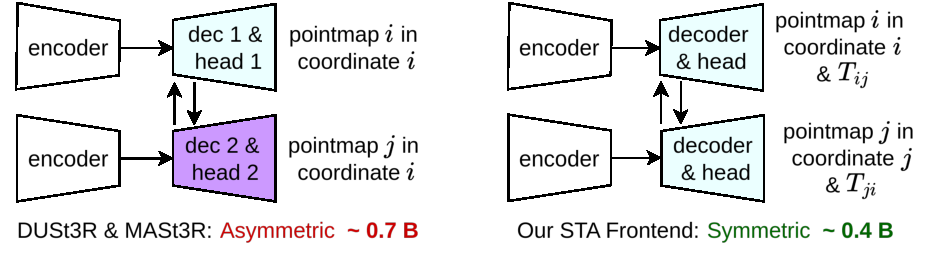
\includegraphics[width=\linewidth]{figs/sym.pdf}
\caption{\textbf{Asymmetric vs. Symmetric Architectures.}
Asymmetric architectures~\cite{dust3r,mast3r} use two decoders to regress point maps in a shared coordinate space. our symmetric formulation regresses relative pose and local point maps with only a single decoder, reducing over 36\% of the parameters ({$\sim$} 0.4 vs. 0.7 billion),  while achieving higher accuracy and enabling pose graph optimization in the backend.}
\label{fig:symmetric}
\vspace{0.5em}
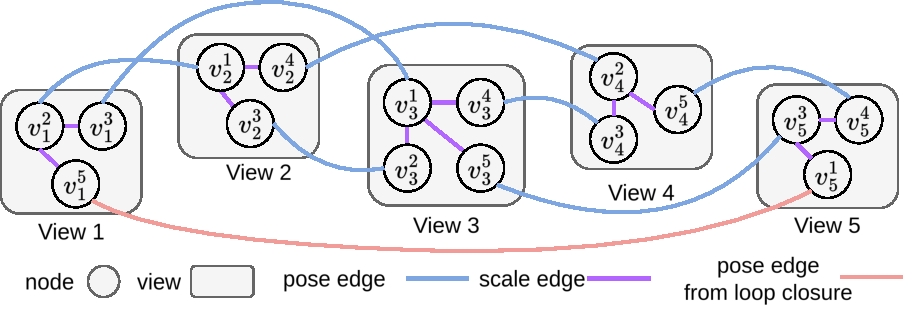
\includegraphics[width=0.9\linewidth]{figs/posegraph.pdf}
\caption{\textbf{An Example Pose Graph for 5 views $(N=2)$.} Nodes of the same view are grouped and connected to the first processed node of that view via \textit{scale edges}. Our two-type-edge design enhances optimization robustness, yielding more accurate poses.}
\label{fig:posegraph}
\vspace{-0.5em}
\end{figure}


\boldparagraph{Geometrical Consistency Loss}
To ensure that the predicted point maps of each pair are spatially consistent when placed in the same coordinate space, we introduce a \textit{geometric consistency loss}.
Given a pair of images with ground-truth intrinsics, depths, and relative poses, each pixel $\bm x$ in view $i$ can be accurately projected into view $j$, yielding its ground-truth corresponding pixel $\bm C_{ij}(\bm{x})$ in view $j$. Then the geometric consistency loss $L_\text{gc}$ is defined as:
\begin{equation}
    L_\text{gc} = \sum_{\bm x \in \bm{I}_{i}} \left\| \bm T_{ij}  \bm P_i(\bm x) - \bm P_j\left( \bm C_{ij}(\bm x) \right) \right\|/n,
\end{equation}
where $\bm T_{ij}$ is the predicted relative transformation and $n$ is the same normalization factor as in \cref{eq:loss_pmap}.

The total training objective function $L$ is the weighted sum of the above three losses,
\begin{equation}
    L = \lambda_\text{pmap}L_\text{pmap} + \lambda_\text{pose}L_\text{pose} + \lambda_\text{gc}L_\text{gc},
\end{equation}
where $\lambda_\text{pmap}$, $\lambda_\text{pose}$ and $\lambda_\text{gc}$ are weighting factors.



\begin{table*}[t]
    \centering
    \vspace{-0.5em}
    % \scriptsize
    \small
    \setlength{\tabcolsep}{8.7pt}
    % \resizebox{2\columnwidth}{!}
    {
    \begin{tabular}{ll|ccccccc|c}
    \toprule
    & Method  & \texttt{chess} & \texttt{fire} & \texttt{heads} & \texttt{office}& \texttt{pumpkin} & \texttt{kitchen} & \texttt{stairs} & \textbf{Avg.}\\
    \midrule
    \cellcolor[HTML]{EEEEEE} & \lo NICER-SLAM~\cite{zhu2024nicer}
    & \lo \textbf{0.033} & \lo 0.069 & \lo 0.042 & \lo 0.108 & \lo 0.200 & \lo 0.039 & \lo 0.108 & \lo 0.086\\
    \cellcolor[HTML]{EEEEEE} & \lo DROID-SLAM~\cite{teed2021droid}
    & \lo 0.036& \lo \textbf{0.027} & \lo 0.025 & \lo \textbf{0.066} & \lo \textbf{0.127} & \lo \textbf{0.040} & \lo 0.026 & \lo \textbf{0.049}\\
    \multirow{-3}{*}{\cellcolor[HTML]{EEEEEE}\rotatebox[origin=c]{90}{\textit{Calib.}}} & \lo GlORIE-SLAM~\cite{zhang2024glorie}
    & \lo 0.036 & \lo 0.029 & \lo \textbf{0.014} & \lo 0.094 & \lo 0.144 & \lo 0.053 & \lo \textbf{0.020} & \lo 0.056\\
    % \lo MASt3R-SLAM~\cite{murai2025mast3rslam}
    %  & \lo 0.053 & \lo \textbf{0.025} & \lo 0.015 & \lo 0.097 & \lo \textbf{0.088} & \lo 0.041 & \lo 0.011 & \lo \textbf{0.047}\\
    %Loopy-SLAM$^*$~\cite{liso2024loopyslam}  & 4.2 & 7.5 & 8.3 & 7.5 & 10.6 & 7.9 & 7.5 & 5.2 & \textbf{7.4}\\
    \midrule
    \cellcolor[HTML]{EEEEEE} & CUT3R~\cite{wang2025cut3r}
    & 0.743 & 0.226 & 0.363 & 0.664 & 0.546 & 0.381 & 0.413 & 0.477\\
    \cellcolor[HTML]{EEEEEE} & SLAM3R~\cite{liu2025slam3r}
    & 0.089 & 0.048 & 0.036 & \nd 0.088 & 0.196 & 0.102 & 0.126 & 0.098\\
    \cellcolor[HTML]{EEEEEE} & MASt3R-SLAM~\cite{murai2025mast3rslam}
    & \nd 0.063 & \rd 0.046 & \rd 0.029 & \rd0.103 & \st 0.112 & \rd 0.074 & \nd 0.032 & \nd 0.066\\
    \cellcolor[HTML]{EEEEEE} & VGGT-SLAM~\cite{maggio2025vggtslam}
    & \st 0.037 & \st 0.026 & \st 0.022 & \rd 0.103 & \rd 0.147 & \nd 0.063 & \rd 0.095 & \rd 0.070\\
    \multirow{-5}{*}{\cellcolor[HTML]{EEEEEE}\rotatebox[origin=c]{90}{\textit{Uncalib.}}} & \textbf{\ours}
    & \rd 0.073 & \nd 0.035 & \nd 0.028 & \st 0.055 & \nd 0.129 & \st 0.035 & \st 0.029 & \st 0.055\\
    \bottomrule
    \end{tabular}
    }
    \caption{
    \textbf{Camera Trajectory Estimation (ATE RMSE) on 7-Scenes~\cite{shotton2013-7scenes}.}
    \ours performs the best on average.
    }
    \label{tab:traj_7scenes}
    \vspace{-1em}
\end{table*}



\subsection{Backend Pose Graph Optimization}
\label{subsec:backend}
\boldparagraph{Notation} In the backend, a $\mathrm{Sim}(3)$ pose graph $\mathcal{G} = (\mathcal{V}, \mathcal{E})$ is maintained and optimized to mitigate accumulated errors introduced by the two-view estimations. The vertex set $\mathcal{V}$ and edge set $\mathcal{E}$ are defined as
\begin{align}
    \mathcal{V} = \{\bm v_i^j\mid i,j \in\mathbb{N} \}, \quad
    \mathcal{E} = \{\bm e_{ij} \mid i,j\in\mathbb{N} \},
\end{align}
 where $\bm v_i^j,\bm e_{ij} \in \mathrm{Sim}(3)$, each vertex $\bm v_i^j$ represents an absolute camera pose with scale, of view $i$, with view $i$ and view$j$ as the input of STA; each edge $\bm e_{ij}$ encodes the relative transformation between a pair of connected vertices $\bm v_i^j$ and $\bm v_j^i$.
 Both $\bm v_i^j$ and $\bm e_{ij}$ have a rigid transformation part $\bm T\in \mathrm{SE}(3)$  and a scale part $s\in\mathbb{R}^+$.

\boldparagraph{Graph Construction}
To construct the pose graph, for a given view $i$, the STA model performs $2N$ forward passes with neighboring views $j \in [i-N, i-1] \cup [i+1, i+N]$. The predicted pointmap for each view in each forward pass corresponds to a node in the graph, resulting in multiple nodes per view since each view is processed multiple times by the frontend model.
As shown in \cref{fig:posegraph}, we define two types of edges in the graph. \textit{Pose edges} connect two nodes generated from the same forward pass, using the estimated relative camera pose and an identity relative scale, based on the assumption that the two local point maps from a single forward pass share the same scale. \textit{Scale edges} connect nodes belonging to the same view but obtained in different forward passes (paired with different neighboring views), with the rigid transformation component set to identity, and the scale component solved via weighted least squares between the predicted point maps of different forward passes.
Among all nodes of the same view, \textit{scale edges} are constructed only between the first processed node and the others for sparsity and simplicity.

\boldparagraph{Loop Closure} We use Bag of Words~\cite{GalvezTRO12} to detect loop candidates, which form new pairs. Then we can feed each candidates pair into our STA model to confirm these proximity. If the predicted confidence score of the relative pose is higher than a predefined threshold $\tau_p$, this pair is accepted as a valid loop, and two new nodes connected by a \textit{pose edge} are added. Each new node is also connected to the first processed node of its corresponding view via a \textit{scale edge}.






\boldparagraph{Optimization}
We perform pose graph optimization using the Levenberg--Marquardt algorithm in the space of Lie algebra $\mathfrak{sim}(3)$.
\begin{equation}
\min_{\{\bm v_i^j \in \mathcal{V}\}} \sum_{\bm e_{ij} \in \mathcal{E}}
\left\|
\log_{\mathrm{Sim}(3)}\left( \bm e_{ij} \cdot ({\bm{v}}_i^j)^{-1}\cdot {\bm{v}}_j^i \right)
\right\|_{\bm \Omega_{ij}}^2
\end{equation}
where $\bm \Omega_{ij}$ represents the covariance matrix, derived from the confidence score predicted by the STA model. The optimization process takes less than 5 iterations to converge in most cases.

Using the optimized camera pose and scale, the reconstructed pointcloud $\tilde{\bm P}_i^j$ in global coordinate is,
\begin{equation}
    \tilde{\bm P}_i^j = s_i^j \bm R_i^j \bm P_i^j + \bm t_i^j,
\end{equation}
where $\bm R_i^j$, $\bm t_i^j$ and $s_i^j$ are the orientation, position, scale of $\bm v_i^j$ respectively. To avoid redundancy, for each view $i$, we only keep the pointcloud with largest confidence among all $\tilde{\bm P}_i^*$ in the final result.
